%%%%%%%%%%%%%%%%%%%%%%%%%%%%%%%%%%%%%%%%%%%%%%%%%%%%%%%%%%%%%%%%%%
%%%%%%%% CPSC 66 SPRING 2021 EXAMPLE REPORT %%%%%%%%%%%%%%%%%%%%%%%%
%%%%%%%% This template is modified from ICML 2014 %%%%%%%%%%%%%%%%
%%%%%%%%%%%%%%%%%%%%%%%%%%%%%%%%%%%%%%%%%%%%%%%%%%%%%%%%%%%%%%%%%%

\documentclass{article}

%include any external packages here.  This is similar to loading a
%library in python or C++

% use Times
\usepackage{times}
% For figures
\usepackage{graphicx}
\usepackage{subfigure}

% For citations
\usepackage{natbib}
% for formulas
\usepackage{amsmath}

% For algorithms and pseudocode
\usepackage{algorithm}
\usepackage{algorithmic}

%Adds hyperlinks to your citations automatically
\usepackage{hyperref}

%for drawing
\usepackage{tikz}


% Packages hyperref and algorithmic misbehave sometimes.  We can fix
% this with the following command.
\newcommand{\theHalgorithm}{\arabic{algorithm}}

\usepackage[accepted]{icml2014}


% If your title is long (below), use this command to also provide
% short version.  This will go on the top of every page
\icmltitlerunning{Final Report}

\begin{document}

\twocolumn[ %use two column if you need a text to span across the whole page
\icmltitle{ CPSC 66 Final Report: \\ % \\ force a new line
RNN Performance Analysis in Language Translation }

\icmlauthor{Wilbert Fundira}{wfundir1@swarthmore.edu}
\icmlauthor{Nelson Dufitimana}{ndufiti1@swarthmore.edu}
\icmlauthor{Kelvin Darfour}{kdarfou1@swarthmore.edu}
\icmlauthor{Bereket Nigussie}{bniguss1@swarthmore.edu}

\vskip 0.3in
]

\begin{abstract}
We explore the application of recurrent neural network models in the field of language translation. Our primary goal is to investigate how different recurrent neural network architectures perform on this task. We implement and compare three types of models: a Simple Recurrent Neural Network (RNN), a Gated Recurrent Unit (GRU) network, and a Long Short-Term Memory (LSTM) network. Each model was trained on a data set comprising English sentences as input and French sentences as targets. The performance of these models was evaluated based on BLEU (Bilingual Evaluation Understudy). Our results indicated that the LSTM model achieved the highest accuracy score of 0.94 and the highest BLEU score of 0.61. While the GRU model had a similar accuracy of 0.94, it achieved a lower BLEU score of 0.57. The Simple RNN, despite its relative simplicity, demonstrated commendable performance with a BLEU score of 0.60 and an accuracy of 0.93. 

\end{abstract}

\section{Introduction}
\label{introduction}

When humans engage with written text, their thoughts persist through the reading. This means that as they transition from one sentence or paragraph to another, their comprehension builds upon prior context rather than starting from scratch. Despite the apparent simplicity of this cognitive task, traditional neural networks lack this capability. The introduction of Recurrent Neural Networks addresses this limitation, incorporating feedback `loops' to facilitate information persistence. However, as the temporal gap widens between the current sentence and the context to be retained, this same task becomes quite
complex for simple RNNs. The introduction of both the  Gated Recurrent Units and the Long Short-Term Memory Networks (LSTMs) seeks to address this challenge.
Both GRUs and LSTMs are advanced types of RNNs, specifically designed to retain long-term dependencies. 
They accomplish this through the use of gates that control 
information flow, enabling them to effectively maintain and
utilize context across extended sequences. The LSTM, in particular, stands out for its capability to handle such problems. Equipped with additional gates and a unique cell state mechanism, LSTMs are adept at preserving even longer dependencies than GRUs. 

With this in mind, we now present our central hypothesis for our work: ``For language translation tasks, we hypothesized that LSTMs will outperform GRUs, and GRUs will outperform simple RNNs." To explore this hypothesis, we leverage TensorFlow's Keras library to implement these 3 models and compare their performance on an English-to-French dataset using accuracy and BLEU score.


\section{Methods}

We first explore the underlying architecture for each 
of the three models and then look at the data we used for
the analysis. 

\subsection{Model Architecture}

\subsubsection{Recurrent Neural Networks}
 Simple RNNs are a class of neural networks designed for processing sequential data, making them ideal for tasks like language translation. In an RNN, connections between nodes form a directed graph along a temporal sequence, allowing it to exhibit temporal dynamic behavior. This architecture enables the network to retain information in 'hidden' layers, which act as memory cells, carrying information across time steps. Figure~\ref{simple-rnn} shows, the underlying mechanism. The output at each time step $x_{t-1}$ is fed in as input into the next time-step $x_{t}$, creating short-term dependencies \cite{Olah15}. However, RNNs are known to struggle with long-term dependencies. As the gap between relevant information and the point where it is needed grows, RNNs tend to lose the ability to learn to connect the information.

 \begin{figure}[ht]
\vskip 0.2in
\begin{center}
\centerline{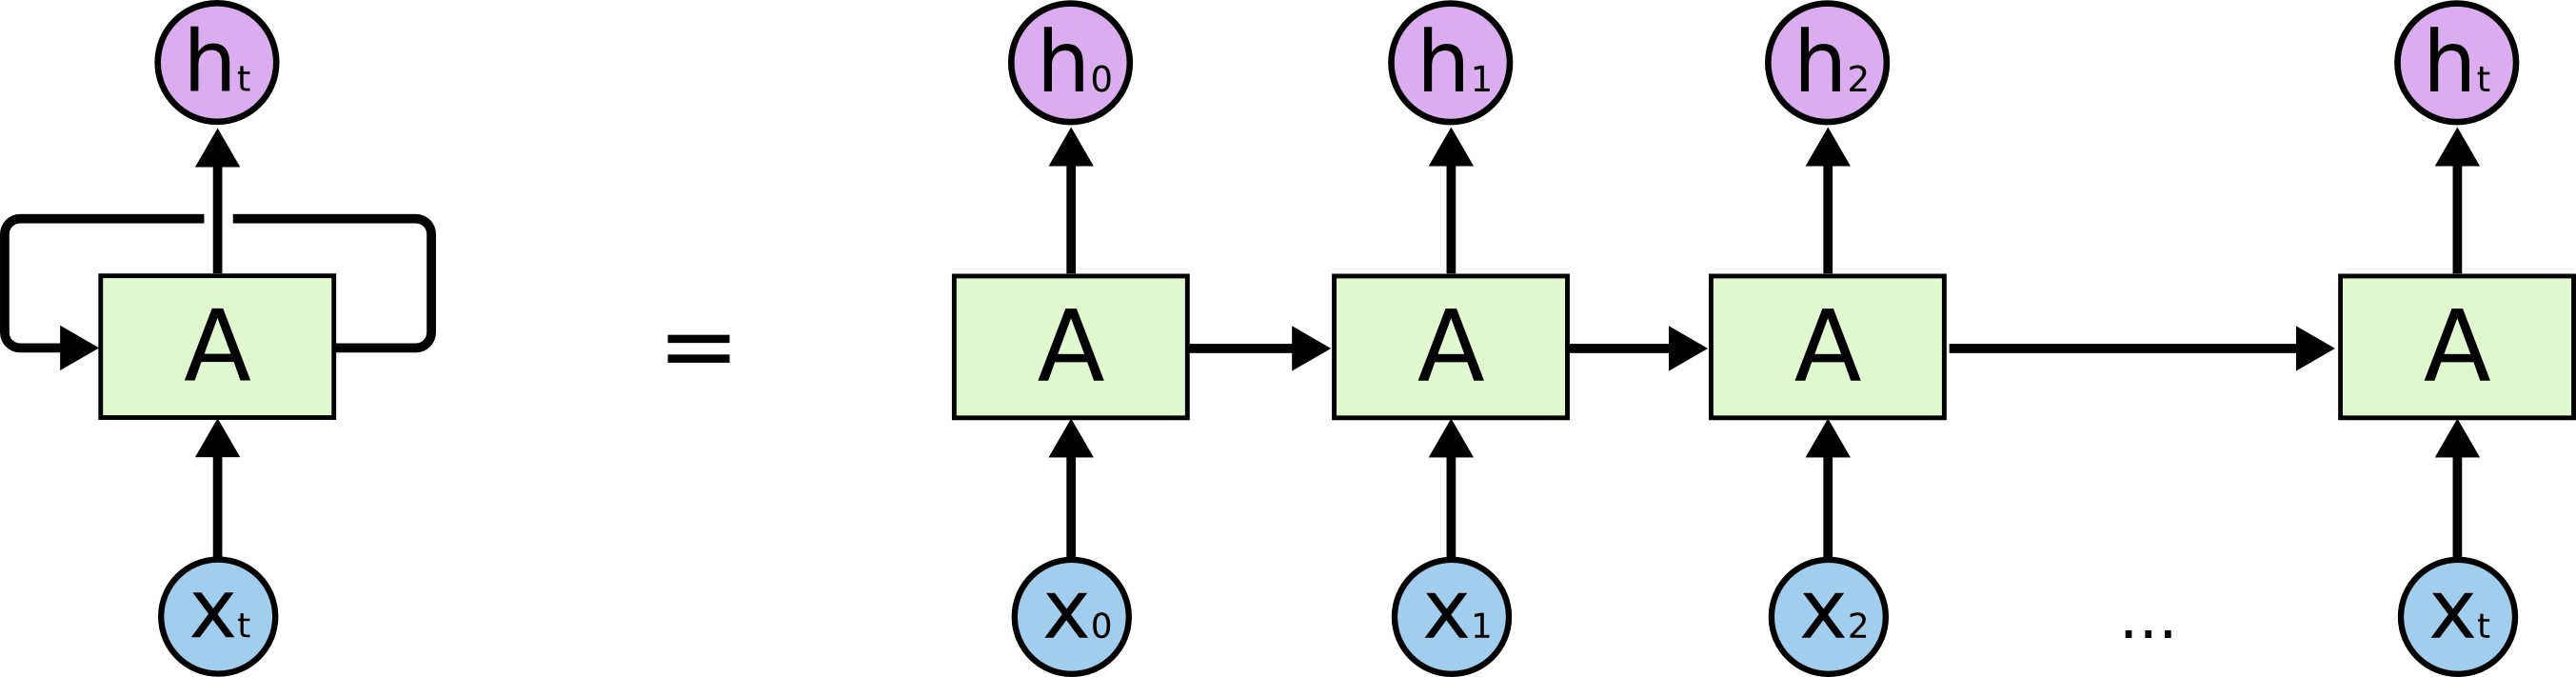
\includegraphics[width=\columnwidth]{ML_images/RNN-unrolled.png}}
\caption{An unrolled simple recurrent neural network.}
\label{simple-rnn}
\end{center}
\vskip -0.2in
\end{figure}

\subsubsection{Gated Recurrent Units}

To address the limitations of RNNs in handling long-term dependencies, we employed Gated Recurrent Units (GRUs). GRUs are a variation of RNNs that include gating mechanisms. These gates – the update and reset gates – decide what information should be passed to the output. The update gate helps the model to determine how much of the past information (from previous time steps) needs to be passed along to the future, while the reset gate decides how much of this past information to forget \cite{Jabreel}. This architecture allows GRUs to better maintain information over longer sequences compared to simple RNNs, making them more effective for tasks where long-term contextual information is important.

\begin{figure}[ht]
\vskip 0.2in
\begin{center}
\centerline{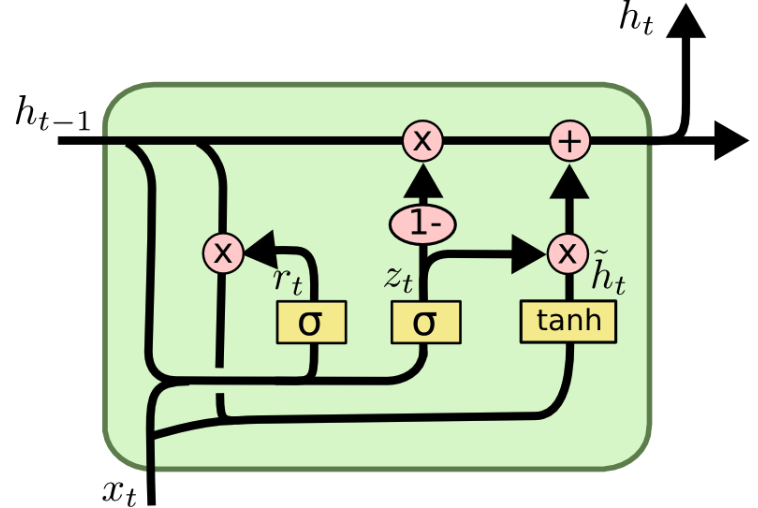
\includegraphics[width=\columnwidth]{ML_images/GRUs.png}}
\caption{One repeating module of a GRU.}
\label{GRU}
\end{center}
\vskip -0.2in
\end{figure}

\subsubsection{Long Short-Term Memory Networks}

 LSTMs are more advanced than simple RNNs and are more or less an extension of GRUs, specifically designed to overcome the problem of long-term dependencies. The key to LSTMs' effectiveness is their cell state and three types of gates: input, output, and forget gates. The cell state acts as a conveyor belt, running straight down the entire network chain, with only minor linear interactions \cite{Olah15}. It’s this ability of the cell state to carry relevant information across many time steps that make LSTMs suitable for tasks requiring the recognition of long-term dependencies. The gates in LSTMs regulate the flow of information into and out of the cell state, thus allowing the network to selectively remember or forget patterns. More specifically, the input gate controls the extent to which a new value flows into the cell state, the forget gate determines what information the cell state should discard and the output gate determines the next hidden state. 
 \begin{figure}[ht]
\vskip 0.2in
\begin{center}
\centerline{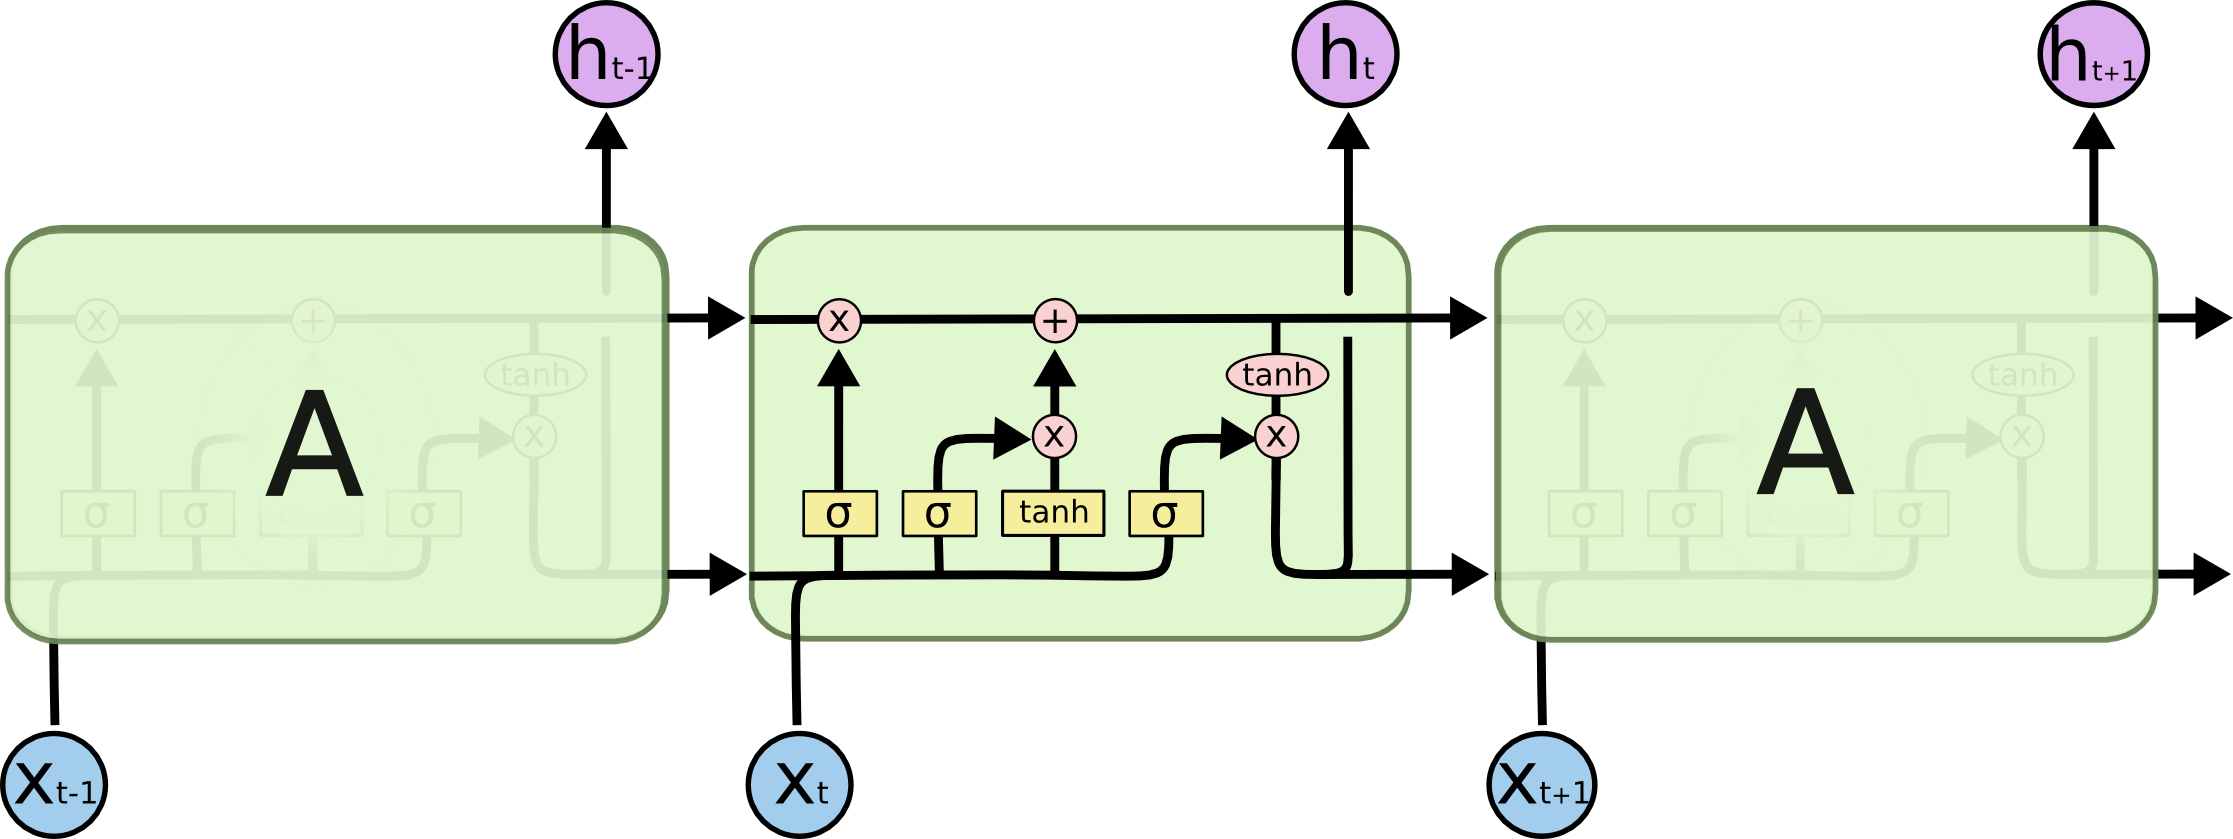
\includegraphics[width=\columnwidth]{ML_images/LSTM.png}}
\caption{One repeating module of an LSTM.}
\label{LSTM}
\end{center}
\vskip -0.2in
\end{figure}


\subsection{Data}

\subsubsection{Down-sampling}

To evaluate the three models, we use a data set from the Tatoeba Project aggregated by ManyThings.org \cite{manythings.org}. Our initial task in data pre-processing involved managing the vocabulary size of our data set to mitigate the challenges that come with working with large language corpora. In language 
translation tasks, a larger vocabulary can significantly impact both the training time and the accuracy of the model. For instance, in a corpus of 4000 words containing 3500 unique words, the high proportion of unique words adds complexity to the learning process because the model ends up getting few examples to learn each word and the context surrounding it adequately. To tackle this, we balance the ratio of unique words to total words by implementing a down-sampling strategy. This involves filtering out less frequent words and setting a frequency threshold to refine our vocabulary. To be specific, we restrict the dataset to only sentences with words that appear $k$ times in the. One can think of this $k$ as a tunable parameter that can be adjusted depending on model complexity and computer resources, among many others. With $k$ set to $500, 000$ our data set was transformed as illustrated in the figures below. The main Venn diagram represents the total number of words in the dataset whereas the inner Venn represents unique words in the dataset.

\begin{figure}[ht]
\begin{tikzpicture}[scale=0.8, transform shape]

  % First set of Venn diagrams
  \begin{scope}
    \node[circle, minimum size=4cm, fill=blue!40] (A) at (0,0) {2.9M};
    \node[circle, minimum size=1.5cm, fill=red!40] (B) at (0,1.25) {16.7K};
  \end{scope}

  % Arrow
  \draw[->, thick] (2.1,0) -- (3.8,0);

  % Second set of Venn diagrams
  \begin{scope}[xshift=6cm]
    \node[text=black,circle, text=black,minimum size=4cm, fill=blue!40] (C) at (0,0) {2.2M};
    \node[text=black,circle, text=black, minimum size=1.5cm, fill=red!40] (D) at (0,1.25) {13.6K};

  \end{scope}



  % Fix the venn diagram to demonstrate downsampling. 
\end{tikzpicture}
      \caption{English Dataset before and after downsampling.}
\end{figure}

\begin{figure}[ht]
\begin{tikzpicture}[scale=0.8, transform shape]

  % First set of Venn diagrams
  \begin{scope}
    \node[circle, minimum size=4cm, fill=blue!40] (A) at (0,0) {3.1M};
    \node[circle, minimum size=1.5cm, fill=red!40] (B) at (0,1.25) {31.8K};
  \end{scope}

  % Arrow
  \draw[->, thick] (2.1,0) -- (3.8,0);

  % Second set of Venn diagrams
  \begin{scope}[xshift=6cm]
    \node[text=black,circle, text=black,minimum size=4cm, fill=blue!40] (C) at (0,0) {2.4M};
    \node[text=black,circle, text=black, minimum size=1.5cm, fill=red!40] (D) at (0,1.25) {24.4K};

  \end{scope}



  % Fix the venn diagram to demonstrate downsampling. 
\end{tikzpicture}
      \caption{French Dataset before and after downsampling.}
\end{figure}


\subsubsection{Tokenization and Padding}
To allow the network to perform linear algebra operations 
on our data, we need to convert it to numerical form. We 
rely on Keras to assign each word in our corpus a unique ID
that is consistent throughout the data set. We apply this process to both the English and French sentences in our dataset, ensuring that each sentence is represented as a sequence of integers corresponding to the words in that sentence. However, this is not enough since sentences are inevitably going to be of varying lengths, which prevents any linear algebra operation on the resulting matrix due to differences in dimensions. To address this, we pad the numerical data with zeros at the very end using the longest sentence that appears in the corpus as a benchmark. This step ensures that all input sequences that go into the model have equal dimensions, which is crucial for efficient and error-free processing by the neural network.

\section{Experimental Results}


\subsection{Experimental Methodology}
% mention softmax function
In training our model, we leverage the Keras library to construct the Simple RNN, GRU, and LSTM models. The core of each model is an Embedding layer, trained from scratch, to transform the integer-encoded sentences into dense word vectors to capture semantic meaning. Depending on the model, we use RNN, GRU, or LSTM layers to process sequential language data, enhanced by Dense layers for learning non-linear feature combinations and Dropout layers to mitigate over-fitting. Each model uses a softmax activation function to provide a one-hot vector encoding to our outputs, which is a common technique in many multi-class labeling tasks in deep learning.  We compile these models using sparse categorical cross-entropy loss function and Adam as the optimizer. The models undergo multiple training epochs, with performance monitored on a validation set, ensuring they effectively learn to translate English to French by capturing linguistic patterns and structures. Before we analyze the results, we look at how the BLEU score is calculated.  
it in our tasks. 

\subsubsection{BLEU Score}

BLEU is a precision-based metric that is widely used 
in Natural Language Processing (NLP) tasks as a performance metric. To quickly go over how BLEU works, let us consider the following two sentences and 
assume that they are related to our model's expected output and
actual output respectively: 



\textbf{Target:} \textcolor{green}{Le gardien est arrivé en retard} \textcolor{red}{car il pleuvait.} 


\textit{\textbf{English Translation:} The guard arrived late because it was raining.}


\textbf{Prediction:} \textcolor{green}{Le gardien est arrivé en retard} \textcolor{red}{à cause de la pluie.} 


\textit{\textbf{English Translation:}The guard arrived late because of the rain.}


In the calculation of the BLEU score, the initial step involves examining how many words match consecutively. In our approach, we limited this to single-word matches, ensuring a straightforward one-to-one correspondence in the 
sentence. Alternatively, it's feasible to consider up to four consecutive matching words in both the prediction and the target. The number of matching 
words is what we call a \textit{N-gram} where N is the number we chose. 

The above two sentences convey the same meaning but use slightly 
different wording as one would expect when it comes to languages. BLEU attempts to score this predicted sentence
based on the idea that ``the closer the predicted sentence is to the human-generated target sentence, the better it is."\cite{Doshi}

Since BLUE is precision-based, we look at the matches in the prediction relative to the total words in the prediction. For the above example, 
we would have a 1-gram precision of $6/11 \approx 0.55$. 

The next step is to get a weighted average using the following formula:
\begin{equation}
\exp\left(\sum_{w=1}^{N} w_n \log p_n\right)
\end{equation}

Where $N=4$ and $p_n$ represents the $n^{th}$ gram precision value. 

The third part involves calculating a ``Brevity Penalty."

We need this score because when relying on precision, it becomes evident that we could generate a predicted sentence comprising a single word, such as ``gardien" or ``est," and the 1-gram Precision would be 1/1 = 1, implying a flawless score. However, this is deceptive as it rewards shorter sentences while penalizing long sentences. 

To counteract this, Bleu needs a form of penalty to avoid rewarding short sentences. The Brevity Penalty does this.
\begin{equation}
Brevity Penalty = 
\left\{
    \begin{array}{lr}
        1, & \text{if } c > r\\
        e^{1-r/c}, & \text{if } c\leq r
    \end{array}
\right\} 
\end{equation}

where $c$ number of words in the predicted 
sentence and $r$ number of words in the target 
sentence.


Finally, one can get the Blue score  by multiplying equations 1 and 2:

$Blue(N) = Brevity Penalty \cdot Geometric average. $



In our approach, we utilize sentence-level BLEU rather than 
corpus-level BLEU, opting for a comparison between sentences 
rather than evaluating the output sentence against our entire
corpus. This choice is motivated by considerations of computational resource usage and runtime efficiency. We calculate the Bleu score for each sentence and compute the average to derive the overall BLEU score for our test set.

\subsection{Results}

In the evaluation of our models, we employ two primary metrics: accuracy, as calculated by Keras, and the BLEU score. Accuracy provides a direct measurement of the model's ability to correctly predict translations, while the BLEU score offers insights into the quality of the translations, comparing them against a reference translation for aspects like fluency and accuracy in word choice.

We summarize our results in Table 1. Our findings reveal that the LSTM model demonstrates superior performance, achieving an accuracy of 0.94 and a BLEU score of 0.61. The GRU model is close behind, also with an accuracy of 0.94 but a slightly lower BLEU score of 0.57. The Simple RNN model, despite its relative simplicity, delivers a robust performance with an accuracy of 0.93 and a BLEU score of 0.60. Additionally, we monitor and plot loss and accuracy curves throughout the training process. From these results, it is very crucial to comment on the high accuracy values and low bleu scores. In the realm of language translation, relying solely on accuracy is not particularly effective for evaluating the performance of language translation models. This is because our model's predictions might omit a word or employ synonyms, neither of which necessarily indicates an incorrect translation. These instances may simply suggest that the model is still in the process of grasping the nuanced usage of certain words. 
For this particular project, it is confusing to understand what accuracy
represents, hence our evaluation emphasizes bleu as the right metric choice.

These visualizations in Figure~\ref{fig:all_curves} provide a clearer understanding of the models' learning progression over epochs, illustrating performance improvements.



\begin{table}[t]
\caption{Accuracy and BLEU Scores for the three models.}
\label{sample-table}
\vskip 0.15in
\begin{center}
\begin{small}
\begin{sc}
\begin{tabular}{lcccr}
\hline
\abovespace\belowspace
Model & Accuracy & BLEU Score \\
\hline
\abovespace
Simple RNN    & 0.93& 0.60 \\
GRU & 0.94& 0.57\\


\belowspace
LSTM   & 0.94&0.61 \\
\hline
\end{tabular}
\end{sc}
\end{small}
\end{center}
\vskip -0.1in
\end{table}



\subsection{Discussion}

It is important to note that the evaluation of translation models is a complex task. While we initially used the inbuilt accuracy metric provided by Keras, we quickly realized its limitations. This metric doesn't fully capture the quality of translation, and we observed instances where the predicted sentence was less than satisfactory but was consistent with what one would expect. In this instance, accuracy might struggle to score the output. This limitation led us to employ the BLEU score, which provides a more comprehensive evaluation by comparing the generated translations to reference translations and factoring in how close the prediction is close to the actual target. BLEU takes into account not only the correctness of the translation but also its fluency and coherence.

One of the most surprising findings from our results was that the Simple RNN outperformed the GRU architecture in terms of both accuracy and BLEU score. Initially, one might expect that more complex models like GRU and LSTM would perform better due to their ability to capture long-term dependencies. However, Simple RNN demonstrated competitive performance, which suggests that for certain language translation tasks, a less complex model may suffice.
On the other hand, it was less surprising that the LSTM model performed the best among the three architectures. LSTMs are specifically designed to handle long-term dependencies through their cell state and gating mechanisms. While there was a concern about the risk of over-fitting, our confidence in the model's performance stemmed from the large amount of training data available. Further improvements may be achieved with additional hyper-parameter tuning, which could lead to even better performance.



\section{Social Implications}
The advancements in machine translation have far-reaching implications in our increasingly interconnected world. Key stakeholders in this realm include global businesses, educational institutions, governmental organizations, and individuals seeking cross-cultural interactions. These entities stand to benefit significantly as machine translation breaks down language barriers, facilitating smoother communication, and fostering international collaboration. For global businesses, accurate and efficient translation tools can lead to more effective marketing strategies, clearer communication with international partners, and access to wider markets. Educational institutions could utilize these advancements to provide more inclusive learning materials and facilitate research collaborations across linguistic boundaries. Governments can improve diplomatic communications and offer better services to linguistically diverse populations.

However, while the benefits are substantial, potential challenges and concerns should not be overlooked. A poor success rate in language translation can lead to the spread of misinformation amongst the key stakeholders. The reliance on machine translation might inadvertently marginalize communities speaking less common languages, as these languages are often underrepresented in training data sets. This could lead to biases in translation quality, perpetuating linguistic inequalities. 

\section{Conclusion} 

In conclusion, our findings emphasize the effectiveness of LSTMs in tasks involving long-term dependencies, such as language translation. Surprisingly, the simpler Simple RNN model outperformed the more complex GRU architecture, challenging our initial expectations.

However, it is imperative to acknowledge the limitations of our experiments. The extensive training time required for our models, approximately 13 hours per run, limited our ability to perform comprehensive hyperparameter tuning. An extension of this project, given ample computing resources and time, would involve fine-tuning hyper-parameters to potentially achieve even better translation accuracy.

Furthermore, there is room for expanding the project by training additional models. For instance, bidirectional implementations of the current models could be explored. Bidirectional models, as the name suggests, process input data in both directions, allowing them to capture contextual information from both past and future inputs. This extension could further enhance translation performance and provide insights into the benefits of bidirectional RNNs.

\section*{Acknowledgments}


We would like to acknowledge and give our warmest thanks to Professor Ben Mitchell for his unwavering support on this project. He was always willing to assist and made several helpful suggestions that contributed to the success of this project.


% In the unusual situation where you want a paper to appear in the
% references without citing it in the main text, use \nocite

\bibliography{references}
\bibliographystyle{icml2014}
%this is driving me nuts!
\appendix
\section{Accuracy Graphs}
\begin{figure*}[htbp]
  \centering
  \includegraphics[width=0.9\textwidth]{ML_images/simpleRNNGraphs.png}
  \hfill
  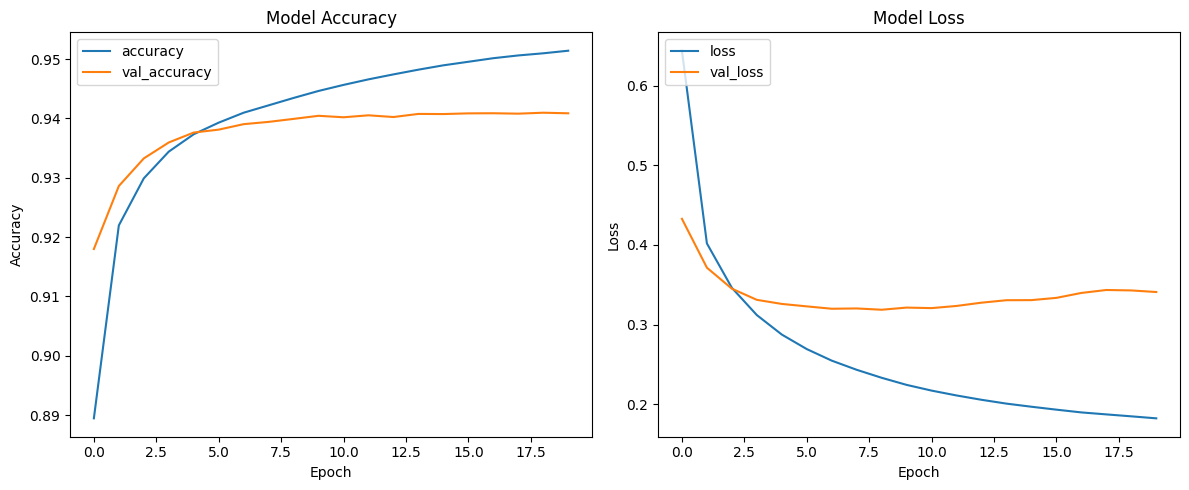
\includegraphics[width=0.9\textwidth]{ML_images/GRUgraphs.png}
  \hfill
  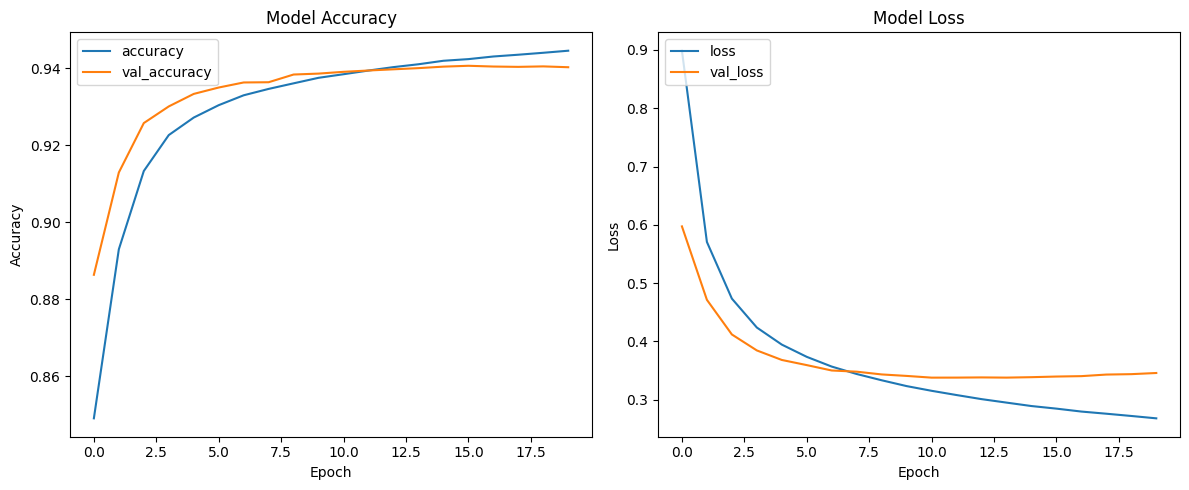
\includegraphics[width=0.9\textwidth]{ML_images/LSTMGraphs.png}
  \caption{Accuracy and loss curves for each model in order: (a) Simple RNN (b) GRU (c) LSTM}
  \label{fig:all_curves}
  \end{figure*}

\end{document}


% This document was modified from the file originally made available by
% Pat Langley and Andrea Danyluk for ICML-2K. This version was
% created by Lise Getoor and Tobias Scheffer, it was slightly modified
% from the 2010 version by Thorsten Joachims & Johannes Fuernkranz,
% slightly modified from the 2009 version by Kiri Wagstaff and
% Sam Roweis's 2008 version, which is slightly modified from
% Prasad Tadepalli's 2007 version which is a lightly
% changed version of the previous year's version by Andrew Moore,
% which was in turn edited from those of Kristian Kersting and
% Codrina Lauth. Alex Smola contributed to the algorithmic style files.